%%% Laboratory	 Notes
%%% Template by Mikhail Klassen, April 2013
%%% Contributions from Sarah Mount, May 2014
%%% Updated by Muhammad Davi, September 2022
\documentclass[a4paper]{tufte-handout}
\usepackage{lab_notes}

\title{Practice Big Data}
\date{2022}

\begin{document}
\maketitle

%%%%%%%%%%%%%%%%%%%%%%%%%%%%%%%%%%%%%%%%%%%%%%%%%%%%%%%%

\begin{projects}
	\begin{description}
		\item [Muhammad Davi, S.Kom., M.Cs.] adalah sebagai dosen pengampu matakuliah practice big data\footnote{Dosen Prodi Teknologi Rekayasa Komputer Jaringan, Jurusan Teknologi Informasi dan Komputer, Politeknik Negeri Lhokseumawe}.
		\item [Peserta dan Kelompok] matakuliah practice big data adalah sebegai berikut:

\begin{table}[!ht]
\caption{Peserta dan Kelompok Matakuliah Practice Big Bata}
\label{tab:peserta}
\centering
\begin{tabular}{ll} 
\toprule
Nama &	Akun Github\\
\midrule
Kelompok 1\\
\midrule
Nadzura Kumaira			& - \\
Nurani Harum Fardaniah	& \url{https://github.com/fardaniahnh} \\
Nuraula Tafiza			& \url{https://github.com/olala17} \\
Nurul Aflah				& \url{https://github.com/Nurulaflahhh} \\
Faiza Yuwafiqi			& \url{https://github.com/faizayuwafiqi} \\
\midrule
Kelompok 2\\
\midrule
Adinda Awaliah			& \url{https://github.com/AdindaAwaliah} \\
Adjie Yusmunandar		& \url{https://github.com/AdjieYusmunandar} \\
Arya Saputra			& \url{https://github.com/AryaSpt} \\
Jihan Dwi Sarah			& \url{https://github.com/jhndsrh} \\
\midrule
Kelompok 3\\
\midrule
Muhammad Munawir		& \url{https://github.com/Munawir027} \\
Muhammad Ikrammullah	& \url{https://github.com/Ikram160302} \\
M. Ikhsan				& \url{https://github.com/Muhammadikhsandev} \\
Zulfahmi				& \url{https://github.com/zulfahmidev} \\
\midrule
Kelompok 4\\
\midrule
\textcolor{red}{Salsabila Irmanda}		& \url{https://github.com/salsalsabilairmanda17} \\
Siti Hajar Al Zahra		& - \\
Syarfani Akbar			& \url{https://github.com/SyarfaniAkbar} \\
Cut Opy Mandalisa		& \url{https://github.com/cutopymdl} \\
\midrule
Kelompok 5\\
\midrule
Rauzatinur Syah			& \url{https://github.com/rauzatinursyah} \\
Resha Russita			& \url{https://github.com/resharussita} \\
Rizki Ilhami			& \url{https://github.com/RIZKIINC} \\
Taravia Fauzah			& \url{https://github.com/traviafzah} \\
\midrule
\end{tabular}
\end{table}
	\end{description}
\end{projects}

%%%%%%%%%%%%%%%%%%%%%%%%%%%%%%%%%%%%%%%%%%%%%%%%%%%%%%%%

\begin{maybe}
    \begin{itemize}
    	\item Matakuliah Practice Big Data
    	\begin{itemize}
    	\item Waktu: 13.30 - 16.00, 16.20 - 18.00\footnote{Istirahat dan Sholat Ashar 20 Menit}
    	\item Ruang: Lab 3\footnote{Lab Jaringan dan Multimedia di Lantai Dasar Gedung Utama}
    	\item Penilaian\footnote{Sesuai ketenuan dari Kepala Lab}
    	\begin{itemize}
    	\item Responsi Kompetensi
    	\item Sikap
    	\item Laporan
    	\item Seminar
    	\item UAS
    	\item Hasil/Benda kerja
    	\end{itemize}
    	\end{itemize}
    	\item Sebelum masuk lab wajib berbaris dan berdo'a terlebih dahulu di depan lab.
    	\item Setiap keluar lab meminta izin kepada dosen pengampu.
    	\item Referensi
    	\begin{itemize}
    		\item Buku Ajar Big Data \citep{Mursyidah2020}.
    	\end{itemize}
    \end{itemize}
\end{maybe}

%%%%%%%%%%%%%%%%%%%%%%%%%%%%%%%%%%%%%%%%%%%%%%%%%%%%%%%%
\clearpage
\newday{8 September 2022}

\newthought{Introduction \& Preparation} \\
Pada pertemuan pertama, kegiatan lab adalah perkenalan dan persiapan kebutuhan untuk praktik big data. Setelah dosen pengampu memperkenalkan diri dan matakuliah yang diajarkan, dilanjutkan perkenalan dari setiap mahasiswa dah hasilnya dapat dilihat pada Tabel \ref{tab:perkenalan}.

\begin{table}[!ht]
\caption{Hasil Perkenalan Mahasiswa}
\label{tab:perkenalan}
\centering
\begin{tabular}{llr} 
\toprule
Nama 	&	Asal Sekolah 	&	Alamat\\
\midrule
Nadzura Kumaira			& & \\
Nurani Harum Fardaniah	& & \\
Nuraula Tafiza			& & \\
Nurul Aflah				& & \\
Faiza Yuwafiqi			& & \\
Adinda Awaliah			& & \\
Adjie Yusmunandar		& & \\
Arya Saputra			& & \\
Jihan Dwi Sarah			& & \\
Muhammad Munawir		& & \\
Muhammad Ikrammullah	& & \\
M. Ikhsan				& & \\
Zulfahmi				& & \\
Salsabila Irmanda		& & \\
Siti Hajar Al Zahra		& & \\
Syarfani Akbar			& & \\
Cut Opy Mandalisa		& & \\
Rauzatinur Syah			& & \\
Resha Russita			& & \\
Rizki Ilhami			& & \\
Taravia Fauzah			& & \\
\end{tabular}
\end{table}

Setelah perkenalan, setiap mahasiswa membuat akun github dan akun discord sebagai media komunikasi dan tempat bekerja secara berkelompok. Hasil dari kegiatan tersebut dapat dilihat pada Tabel \ref{tab:peserta} dan Server Discord pada alamat \url{https://discord.gg/V32EWUx6}.

Tugas di pertemuan pertama adalah menyiapkan \textit{environment} untuk tempat kerja minimal sebagai berikut:
\begin{itemize}
\setlength\itemsep{0em}
\item \textit{Operating System}: Ubuntu 22.04 LTS
\item Processor 2 GHz dual-core
\item RAM sebesar 4 GB
\item Harddisk kosong 25 GB
\item Resolusi layar 1024x768
\end{itemize}
\hrulefill

%%%%%%%%%%%%%%%%%%%%%%%%%%%%%%%%%%%%%%%%%%%%%%%%%%%%%%%%
\clearpage
\newday{15 September 2022}

\newthought{Instalasi Apache Hadoop} \\
Pada pertemuan kedua ini kegiatan yang dilakukan adalah menginstall Apache Hadoop pada \textit{environment} yang telah dibuat pada. Untuk menginstall Apache Hadoop dapat mengikut langkah-langkah berikut ini:
\begin{enumerate}
\item Install Java \\
{\tt sudo apt update} \\
{\tt sudo apt install openjdk-8-jdk -y} \\

\item Verifikasi Instalasi Java \\
{\tt java -version} \\
Hasil verifikasi  instalasi java dapat dilihat pada Gambar \ref{gam:java-version}.
\begin{figure}
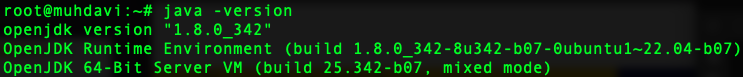
\includegraphics[width=\textwidth]{java-version}
\caption{Mengecek Versi Java}
\label{gam:java-version}
\end{figure}

\item Setup JAVA\_HOME dan JRE\_HOME Variabel
{\tt sudo nano /etc/profile} \\
\begin{lstlisting}
JAVA_HOME=/usr/lib/jvm/java-8-openjdk-amd64
PATH=$PATH:$HOME/bin:$JAVA_HOME/bin
export JAVA_HOME
export JRE_HOME
export PATH
\end{lstlisting}

\item Download Apache Hadoop \\
{\tt wget https://dlcdn.apache.org/hadoop/common/hadoop-3.3.4/hadoop-3.3.4.tar.gz}

\item Ekstrak Apache Hadoop \\
{\tt tar -xzvf hadoop-3.3.4.tar.gz }
\begin{itemize}
\item x $\Rightarrow$ ekstrak file arsip.
\item z $\Rightarrow$ filter file arsip melalui gzip.
\item v $\Rightarrow$ menampilkan proses.
\item f $\Rightarrow$ nama file arsip.
\end{itemize}

\item Pindahkan hasil ekstrak ke /opt/ \\
{\tt sudo mv hadoop-3.3.4 /opt/}

\item Edit file hadoop-env.sh \\
{\tt cd /opt/} \\
{\tt sudo nano hadoop-3.3.4/etc/hadoop/hadoop-env.sh} \\
{\tt export JAVA\_HOME=/usr/lib/jvm/java-8-openjdk-amd64} \\
Untuk mengubah file {\tt hadoop-env.sh} dapat dilihat pada Gambar \ref{gam:java-hadoop}.

\begin{figure}
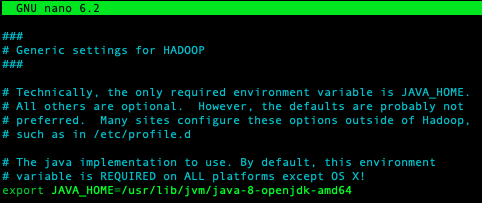
\includegraphics[width=\textwidth]{java-hadoop}
\caption{Konfigurasi Java Home}
\label{gam:java-hadoop}
\end{figure}

\item Verifikasi Hadoop \\
{\tt ./hadoop-3.3.4/bin/hadoop version} \\
Jika instalasi hadoop sudah berhasil, maka ketika mengecek versi hadoop akan muncul seperti yang diperlihatkan pada Gambar \ref{gam:hadoop-version}.

\begin{figure}[!ht]
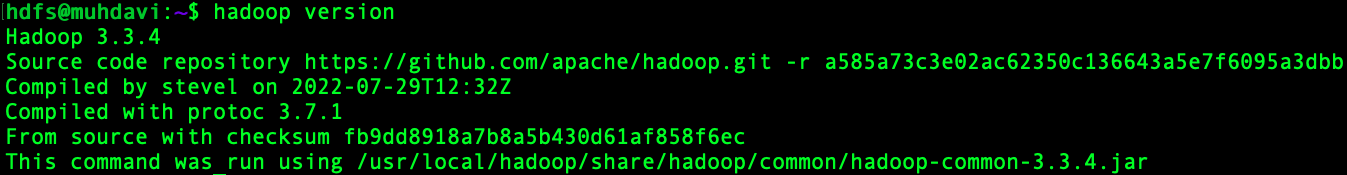
\includegraphics[width=\textwidth]{hadoop-version}
\caption{Mengecek Versi Hadoop}
\label{gam:hadoop-version}
\end{figure}
\end{enumerate}

\hrulefill

%%%%%%%%%%%%%%%%%%%%%%%%%%%%%%%%%%%%%%%%%%%%%%%%%%%%%%%%
\clearpage
\newday{22 September 2022}
\textit{N.B.: Setiap mahasiswa membuat laporan hasil praktikum dengan format yang telah ditentukan. Template laporan dapat di download pada alamat \url{https://github.com/muhdavi/laporan-practice-big-data}.}

\newthought{Instalasi Apache Pig} \\

\section{Laporan Mahasiswa}
\begin{enumerate}
\item Nadzura Kumaira		\\
\textit{isi laporan}
\item Nurani Harum Fardaniah\\
\textit{isi laporan}
\item Nuraula Tafiza		\\
\textit{isi laporan}
\item Nurul Aflah			\\
\textit{isi laporan}
\item Faiza Yuwafiqi		\\
\textit{isi laporan}
\item Adinda Awaliah		\\
\textit{isi laporan}
\item Adjie Yusmunandar		\\
\textit{isi laporan}
\item Arya Saputra			\\
\textit{isi laporan}
\item Jihan Dwi Sarah		\\
\textit{isi laporan}
\item Muhammad Munawir		\\
\textit{isi laporan}
\item Muhammad Ikrammullah	\\
\textit{isi laporan}
\item M. Ikhsan				\\
\textit{isi laporan}
\item Zulfahmi				\\
\textit{isi laporan}
\item Salsabila Irmanda		\\
\textit{isi laporan}
\item Siti Hajar Al Zahra	\\
\textit{isi laporan}
\item Syarfani Akbar		\\
\textit{isi laporan}
\item Cut Opy Mandalisa		\\
\textit{isi laporan}
\item Rauzatinur Syah		\\
\textit{isi laporan}
\item Resha Russita			\\
\textit{isi laporan}
\item Rizki Ilhami			\\
\textit{isi laporan}
\item Taravia Fauzah		\\
\textit{isi laporan}
\end{enumerate}


\hrulefill

%%%%%%%%%%%%%%%%%%%%%%%%%%%%%%%%%%%%%%%%%%%%%%%%%%%%%%%%
\newpage
\bibliographystyle{plain}
\bibliography{lab_notes}

\end{document}

\begin{comment}
\section{Laporan Mahasiswa}
\begin{enumerate}
\item Nadzura Kumaira		\\
\textit{isi laporan}
\item Nurani Harum Fardaniah\\
\textit{isi laporan}
\item Nuraula Tafiza		\\
\textit{isi laporan}
\item Nurul Aflah			\\
\textit{isi laporan}
\item Faiza Yuwafiqi		\\
\textit{isi laporan}
\item Adinda Awaliah		\\
\textit{isi laporan}
\item Adjie Yusmunandar		\\
\textit{isi laporan}
\item Arya Saputra			\\
\textit{isi laporan}
\item Jihan Dwi Sarah		\\
\textit{isi laporan}
\item Muhammad Munawir		\\
\textit{isi laporan}
\item Muhammad Ikrammullah	\\
\textit{isi laporan}
\item M. Ikhsan				\\
\textit{isi laporan}
\item Zulfahmi				\\
\textit{isi laporan}
\item Salsabila Irmanda		\\
\textit{isi laporan}
\item Siti Hajar Al Zahra	\\
\textit{isi laporan}
\item Syarfani Akbar		\\
\textit{isi laporan}
\item Cut Opy Mandalisa		\\
\textit{isi laporan}
\item Rauzatinur Syah		\\
\textit{isi laporan}
\item Resha Russita			\\
\textit{isi laporan}
\item Rizki Ilhami			\\
\textit{isi laporan}
\item Taravia Fauzah		\\
\textit{isi laporan}
\end{enumerate}
\end{comment}
